\chapter{Choix techniques}

Dans cette partie nous cherchons à décrire dans un premier temps les divers choix techniques et spécificités du projets plus en détail.

\section{Analyse Syntaxique}

\subsection{Génération du parseur avec Grammatica}

Comme présenté dans la première partie, l'outil utilisé pour réaliser l'analyse syntaxique d'une formule est Grammatica 1.6. Ce programme écrit en Java est un générateur de parseur en Java et C\#, autrement dit il prend en entrée un fichier texte décrivant les règles d'une syntaxe à suivre et produit 4 classes vers le langage cible.
Ce fichier texte décrivant la grammaire (fournis en annexe) est constitué de deux blocs :
\begin{itemize}
	\item Les tokens, ce sont toutes les chaînes de caractères qui seront acceptées par le parseur.
	\item La production qui est l'ensemble des règles qui articulent les tokens définis précédemment.
\end{itemize}
Les règles définies dans la production doivent être judicieusement écrites afin que la rédaction d'une formule soit suffisamment souple (éviter de forcer l'utilisateur à écrire trop de parenthèse inutile par exemple) mais respecte toujours les règles des formules de la logique. De plus Grammatica, comme beaucoup d'autre générateurs de parseur libres de droits, examine la chaîne de caractère de gauche à droite lors de l'analyse. Cette contrainte empêche d'écrire des règles directement récursives. Par exemple, bien qu'elle soit la plus intuitive on ne peut pas écrire une telle règle :
\newline \begin{center}$Formule \; = \; Formule \; ET \; Formule$\end{center}
car Grammatica bouclera lors de l'analyse. La première solution pour contourner le problème est d'introduire un caractère intermédiaire :
\newline \begin{center}$Formule \; = \; '(' \; Formule \; ET \; Formule  \; ')'$\end{center}
Cette solution bien qu'efficace oblige l'utilisateur à écrire un nombre inutile de parenthèses dans certaines situations, par exemple la formule logique :
\newline \begin{center}$Rose(x) \land est\_grand(x) \land a\_l\_est(x)$\end{center}
devra s'écrire :
\newline \begin{center}$(Rose(x) \land (est\_grand(x) \land (a\_l\_est(x))))$\end{center}
Pour cela on définit une règle spécialement dédiée aux prédicats. Les prédicats étant des cas terminaux de notre récursion on peut écrire :
\newline \begin{center}$Formule \; = \; Predicat \; ET \; Predicat$\end{center}

Une fois que la grammaire est correctement définie, on lance Grammatica afin de générer les quatre classes C\# suivantes :
\begin{itemize}
	\item \textbf{LogicalConstants.cs} qui est une énumération de tous les tokens.
	\item \textbf{LogicalTokenizer.cs} qui fait l'association entre la chaîne de caractères d'un token et la représentation interne propre à Grammatica.
	\item \textbf{LogicalParser.cs} et \textbf{LogicalAnalyzer.cs} qui permettent d'effectuer l'analyse proprement dite d'une chaîne de caractères.
\end{itemize}
Ces quatre classes permettent d'obtenir un arbre syntaxique à partir d'une chaîne de caractères. Cependant cet arbre est représenté selon la bibliothèque de Grammatica et ne correspond pas exactement à la représentation dont on en a besoin. Il est donc nécessaire de parcourir une fois l'arbre afin de le reconstruire avec la représentation propre à notre projet, afin de pouvoir l'utiliser avec un jardin et vérifier l'intégrité de la formule. C'est le rôle des classes \textbf{Formule.cs} et \textbf{FormuleFactory.cs}. Pour résumer, l'analyse syntaxique d'une formule se fait comme suit :

\begin{center}
\begin{figure}[!h]
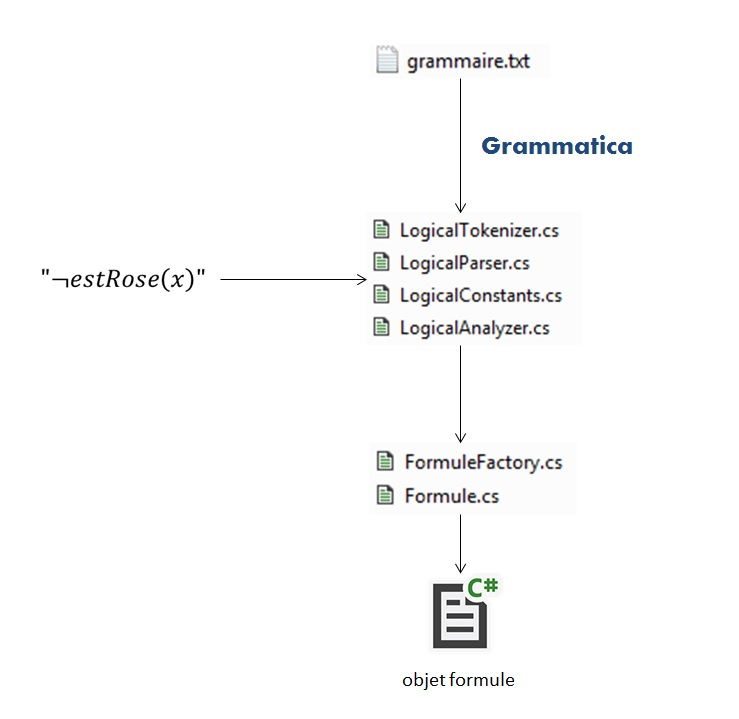
\includegraphics[scale=0.5]{choix_techniques/analyse_syntaxique.jpg}
\caption{Vérification syntaxique avec Grammatica}
\end{figure}
\end{center}
\clearpage

\subsection{Communication avec le script Python}

Comme évoqué précédemment, la brique de base du projet se séparait en deux problématiques distinctes, la grammaire et la communication inter blocs. Nous allons aborder ici ce second point.
\begin{center}\textbf{Fonctionnement}\end{center}
La première problématique amenée par le projet était de pouvoir faire communiquer deux langages différents ensemble.
Après quelques recherches, il s'est avéré qu'une implémentation de Python avait été réalisée spécifiquement pour le développement .NET et Mono, écrit en C\# et donc parfaitement compatible avec Unity 5: IronPython.
Le but était de pouvoir embarquer la solution dans Unity afin que celui-ci puisse gérer par la suite la conversion du projet pour les plateformes Linux, Mac et Windows.
IronPython permet l'utilisation de toute la bibliothèque Python mais avec les avantages du .Net, il est donc possible de faire des appels de fonction directement depuis le C\# sans avoir à passer par des sockets ou autre connecteur réseau. 
De même il est également possible de passer des objets C\# vers Python et inversement, il est alors possible de faire des appels de méthode sur les objets C\# depuis le Python.
Une fois le problème du choix de technologie réglé, il est temps de se questionner sur la manière dont la brique de communication doit agir.
Dans un premier temps, elle est composée d'une méthode principale visée à être appelée par des événements placés sur l'interface utilisateur. Son but et de faire le lien entre les différentes étapes de vérification, en premier lieu le but est d'envoyer la formule à l'analyse syntaxique qui étudie si oui ou non, la formule peut être envoyée à la vérification par le script Python.
Dans le cas où la formule est juste, la brique de communication récupère de l'analyseur la formule modifiée en objet C\# et la renvoie dans une méthode intermédiaire récursive, visant à la retransformer pour qu'elle puisse être lue par le script Python, auquel elle est envoyée au final.
La brique de communication fini son travail en retournant à l'interface utilisateur le résultat du traitement de la formule. Soit un booléen, soit un message d'erreur dans le cas où un problème serait survenu au cours du traitement (mauvaise syntaxe, objet inexistant dans le jardin de base, etc. )

\begin{center}\textbf{Problèmes rencontrés}\end{center}
Lors de la réalisation du cahier des charges et de l'analyse de l'existant, il a été fourni aux deux groupes travaillant sur ce projet deux scripts distincts. Un script en Python et un script en Ocaml.
Notre groupe a choisi de prendre le second. Le premier gros problème rencontré sur la partie communication a été de réussir à trouver comment faire une liaison entre du C\# et de l'Ocaml.
Une seule API fournissant la solution a été trouvée: CSML. Il s'est avéré que la solution n'était plus maintenue depuis plusieurs années et que le projet n'était pas fonctionnel sous des machines en 64 bit. Les nombreuses contraintes et bugs rencontrés lors des tests nous ont fait abandonner très vite cette solution.
Il a alors été abordé l'idée de communiquer via Sockets, cependant nous avons rencontré des erreurs dans la documentation même d'Ocaml nous avons préféré abandonner totalement l'idée de continuer avec Ocaml et nous rabattre sur Python, plus simple à prendre en main rapidement et avec une communauté plus nombreuse derrière.

\newpage{}


\section{L'interface graphique avec Unity}

L'interface graphique est le point central de ce projet. Aussi, le choix du bon langage et/ou du bon outil pour la concevoir fut un choix crucial pour mener à bien ce projet.

\begin{center}
\begin{figure}[!h]
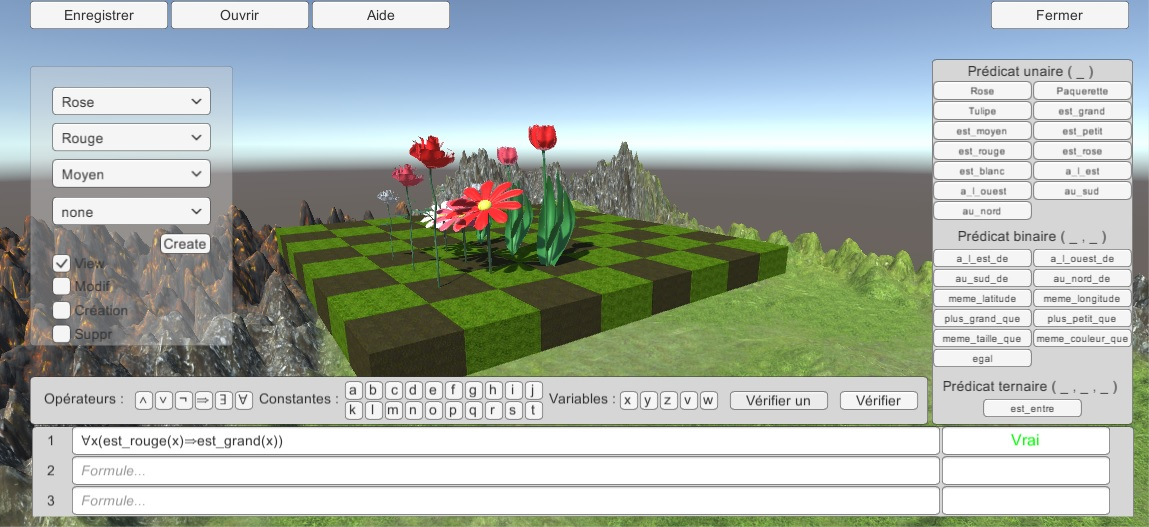
\includegraphics[scale=0.5]{choix_techniques/rendu_final.jpg}
\caption{Rendu final de l'interface graphique}
\end{figure}
\end{center}
\clearpage

\subsection{Présentation et architecture générale}
Notre choix s'est porté sur le moteur de jeux Unity 5 qui, grâce à de nombreux outils performants permet de créer une interface graphique élégante et robuste. Bien que Unity prenne en charge le temps réel, pour notre application nous avions seulement besoin d'utiliser la programmation par évènements. Le bloc qui effectue la liaison entre le code nécessaire à la vérification d'une formule avec un jardin et l'interface graphique en elle-même est donc constitué d'un ensemble de scripts. Ces scripts sont attachés à différents éléments de l'interface graphique (bouton, fleur, formulaire) et sont appelés lorsque l'utilisateur déclenche un évènement attendu. Un script, une fois activé, peut alors soit modifier directement un élément de l'interface graphique (par exemple déplacer ou modifier l'aspect d'une fleur) ou faire appel à un autre script encapsulant le code nécessaire au traitement d'une formule et d'un jardin (vérification, sauvegarde ou chargement de formules et de jardins). De plus on peut diviser les scripts en trois catégories :
\begin{itemize}
\item Les scripts qui n'interagissent qu'avec le clavier et les formulaires, s'occupant de faciliter la rédaction d'une ou plusieurs formules.
\item Les scripts propres au jardin et aux fleurs permettent de positionner et modifier des fleurs dans le jardin.
\item Les scripts liants les deux groupes précédents sont notamment les scripts attachés aux boutons 'Vérifier', 'Vérifier un', 'Sauvegarder', 'Charger' qui sont en charge de récupérer le jardin et les formules pour effectuer différents traitement.
\end{itemize}

L'architecture globale de l'interface graphique peut être schématisée comme suit :

\begin{center}
\begin{figure}[!h]
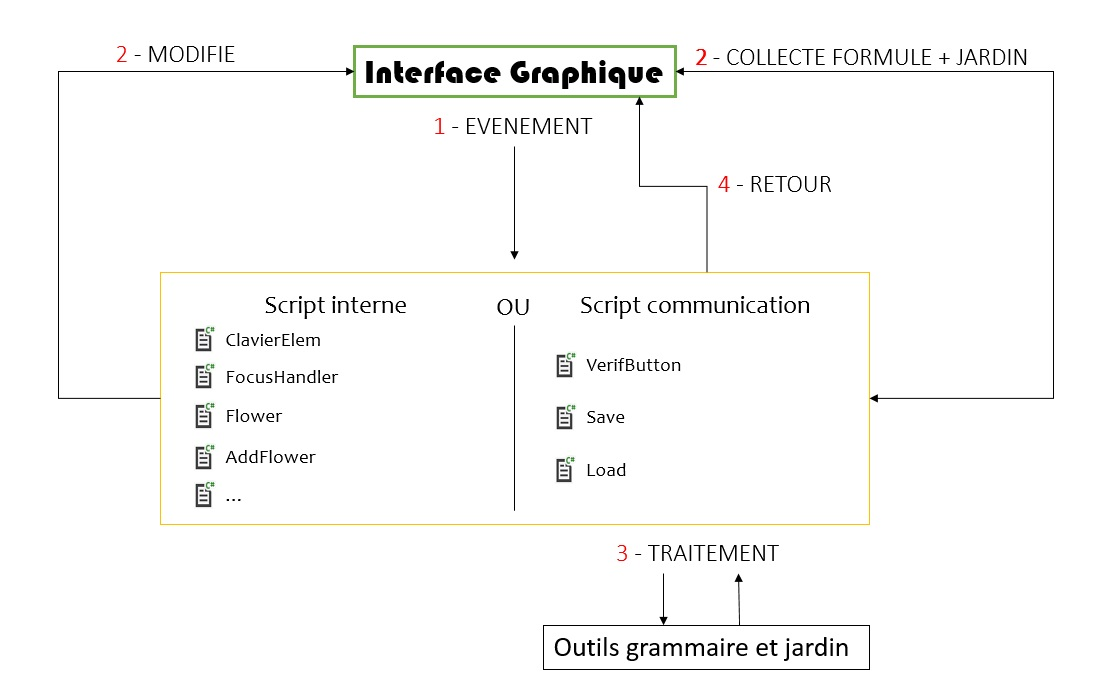
\includegraphics[scale=0.5]{choix_techniques/unity1.jpg}
\caption{Vérification syntaxique avec Grammatica}
\end{figure}
\end{center}
\clearpage

\subsection{Fonctionnement du clavier et des formulaires}

Pour écrire une formule l'utilisateur a 30 formulaires à sa disposition. Ces formulaires fonctionnent avec un clavier virtuel permettant à l'utilisateur de saisir les caractères spéciaux représentant les opérateurs ainsi que les constantes, variables et prédicats afin d'éviter les erreurs de syntaxe bête lors de la réalisation d'une formule. Bien que le fonctionnement du clavier puisse sembler trivial à première vue quelques problèmes furent posés lors de sa conception. En effet, quand l'utilisateur manipule le clavier, au-delà du fait d'ajouter le ou les caractère(s) au formulaire, il faut se souvenir quel formulaire a été sélectionné en dernier et pour chaque formulaire quelle était la position du curseur. Ceci est le rôle des scripts $CaretPos$ et $FocusHandler$. Chaque formulaire possède une instance de $CaretPos$ qui, dans une variable locale, sauvegarde chaque changement du curseur pour se formulaire. Le curseur peut aussi bien être déplacé par un clic de souris que par une édition. $FocusHandler$ au contraire n'est instancié qu'une seule fois dans un panel encapsulant l'ensemble des formulaires. Quand un formulaire est sélectionné à la souris, celui-ci se charge d'appeler une fonction de $FocusHandler$ pour indiquer qu'il est le nouveau formulaire actuellement sectionné. Ainsi, quand l'utilisateur appuie sur un des boutons du clavier virtuel, ce bouton demande au $FocusHandler$ à quel formulaire envoyer la chaîne de caractères. Le formulaire ajoute ensuite les caractères à la bonne position grâce à $CaretPos$.

\subsection{Le jardin et les fleurs}

Le soucis de cette partie était d'arriver à gérer trois comportements différents de l'application sur une même zone, à savoir l'ajout de fleur, la modification de fleurs et leur suppression.
Comme évoqué plus haut, Unity offre une méthode \textit{Update}, si celle-ci est vide, elle est ignorée par le moteur graphique. Cependant si elle est utilisée, elle est alors appelée une fois par \textit{frame} et simule donc une boucle.
Nous avons donc utilisé le plateau afin d'y placer un script de gestion des modes, vérifiant à chaque frame l'état de la boucle et la position de la souris.
Récupérer l'objet que la souris survole est en général simple depuis l'objet lui même, Unity offrant une méthode toute faite. Cependant récupérer ce même objet depuis un autre script, non directement lié, est légèrement plus complexe. Dans ce cas il faut utiliser un \textit{Raycast}, qui est un rayon envoyé depuis la souris sur une ligne droite dont l'angle et la distance max sont fixés dans la méthode offerte par le moteur de jeu. Tout objet n'appartenant pas à la classe d'interface graphique de Unity est alors retourné: c'est le cas des tuiles de notre jardin.
\newline
Les différents modes vont donc offrir un panel de fonctionnalités différent. Le principe de base étant le même pour l'ajout et la modification d'une fleur. Le but est de récupérer les différentes informations des boutons et de les enregistrer dans un objet. Ensuite la boucle principale analyse l'endroit que le pointeur vise et récupère l'objet en question si il fait partie du jardin. On demande alors à la case de créer une visualisation de la fleur que l'on veut. Dans le cas où l'utilisateur est d'accord sur l'emplacement et qu'il clique, on set alors la fleur à l'endroit voulu. Si jamais l'utilisateur préfère une case voisine, alors la visualisation est détruite et reconstruite dans la nouvelle case choisie.
\newline
Chaque ajout et chaque modification est enregistré dans le script du jardin destiné à l'analyse finale.
\newline
L'idée est ici d'utiliser la puissance du moteur graphique, initialement conçu pour les jeux vidéos, capable de gérer la modélisation et la suppression rapide d'objets 3D.
\begin{center}\textbf{Problèmes rencontrés}\end{center}
Dans un premier temps il avait été évoqué de pouvoir générer dynamiquement un aperçu de la fleur dans un menu, et de glisser avec la souris celle-ci du panel vers le plateau. Le soucis de cette méthode était que nous n'avions pas pris en compte la difficulté de pouvoir jongler sur plusieurs plans, les panel étant considérés comme des éléments graphiques 2D contrairement au plateau considéré comme un élément 3D. Arriver à jongler entre les deux axes ainsi que de passer d'un objet 2D à un 3D était trop compliqué.
Il a donc été décidé de se rabattre sur une solution plus simple: installer un système de modes via un menu.
Un autre soucis a été d'arriver à prendre en compte le fait que l'on ne peut pas avoir une même constante sur plusieurs fleurs, il a donc fallut ajouter un système de vérification à la structure déjà en place.

\subsection{Options supplémentaires}

En plus des fonctionnalités de base qui permettent de manipuler un jardin et d'écrire des formules, il est intéressant que l'utilisateur puisse sauvegarder ces deux éléments pour pouvoir les réutiliser plus tard. Dans un premier temps il a fallut définir un format de sauvegarde. Notre choix s'est porté sur un unique fichier contenant deux parties : une pour le jardin et l'autre pour les formules. Le jardin est sauvegardé comme une liste de quintuplets suivant :
\begin{center}$ coordX, coordY, espece, taille, couleur, nom $ \end{center}
et les formules sont simplement des chaînes de caractères recopiées telles quelles. Unity ne possédant pas d'utilitaire graphique pré-fait pour parcourir une arborescence de fichier, il a été nécessaire de reconstruire la notre. Elle se compose simplement de deux champs, l'un indiquant le chemin complet et le nom du fichier destination et l'autre permettant de se déplacer dans l'arborescence du répertoire courant. La figure suivante présente l'utilisation de cet utilitaire :

\begin{center}
\begin{figure}[!h]
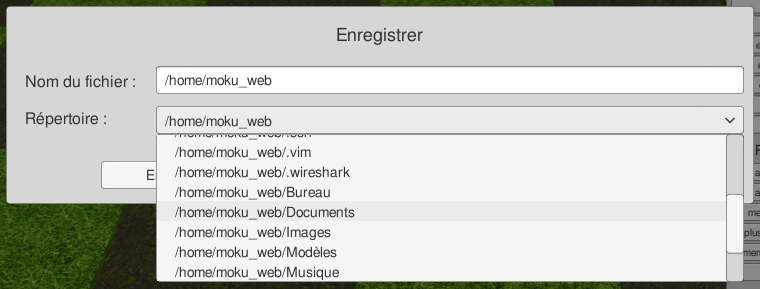
\includegraphics[scale=0.5]{choix_techniques/parcours_rep.jpg}
\caption{Exemple d'utilisation de la fenêtre d'enregistrement}
\end{figure}
\end{center}
\clearpage